%        File: report.tex
%     Created: Sun Feb 21 08:00 AM 2016 E
% Last Change: Sun Feb 21 08:00 AM 2016 E
%
\documentclass[a4paper]{article}

\usepackage[a4paper, margin=1.25in]{geometry}

\usepackage{mathtools} 
\usepackage{amsmath}
\usepackage{amssymb}
\usepackage{newlfont}
\usepackage{caption}
\usepackage{subcaption}
\usepackage{titlesec}
\usepackage{graphicx}
\usepackage{empheq}

\newcommand{\eref}[1]{Eq.~(\ref{#1})}
\newcommand{\erefs}[2]{Eq.s~(\ref{#1}-\ref{#2})}
\newcommand{\pd}[2]{\frac{\partial #1}{\partial #2}}
\newcommand{\pnd}[3]{\frac{\partial^{#3} #1}{\partial #2^{#3}}}

\title{Written Preliminary Exam \#1 \break
       Prepared by Dr. Hassan}

\author{ Kyle B. Thompson }

\begin{document}
\maketitle

\begin{enumerate}
  \item Constant density flow and incompressible flow are two different things.
    Constant density implies that a fluid(s) density is constant, but capable of
    changing (through compression or expansion), whereas incompressible implies
    the fluid(s) density is incapable of changing but that the density in the
    flow is not constant.  A good example from the MAE 550 course to distinguish
    the two is stagnant air in a room, versus an oil/water mixture.  Stagnant
    air in a room is at constant density, but is certainly capable of both
    compression or expansion; therefore, it is a constant density flow, but not
    incompressible.  An oil/water mixture is not constant density.  As
    illustrated in figure \ref{fig:incompressible},the
    water and oil are different fluids with different densities, but the fluids
    are incompressible because both the water and oil are not capable of
    compression or expansion (at least in a practical sense); therefore, it is
    not a constant density flow, but it is incompressible.

    \begin{figure}[h]
      \centering
      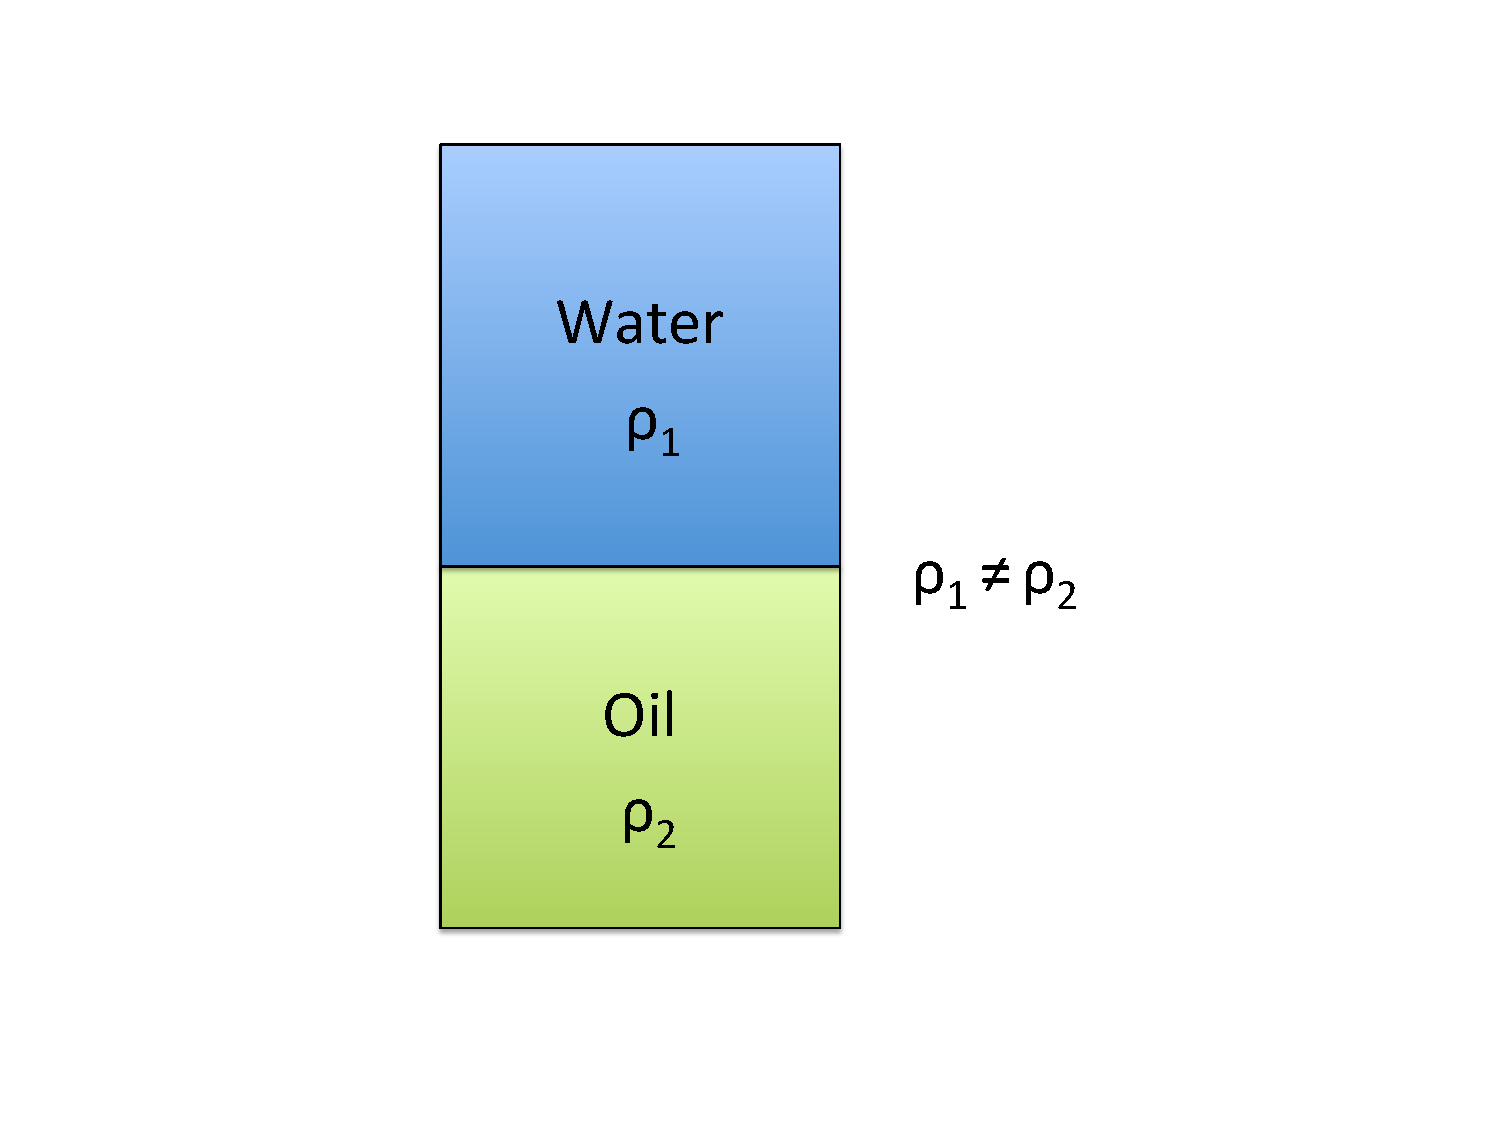
\includegraphics[width=0.8\textwidth,trim={0 2cm 0 2cm},clip]{oil_water_fig}
      \caption{Incompressible Fluid Flow Example}
      \label{fig:incompressible}
    \end{figure}

  \item The Pohlhausen method is typically defined as a velocity profile polynomial
    \begin{equation}
      \begin{gathered}
        \frac{u}{U_e} = a + b\eta + c\eta^2 + d\eta^3 + e\eta^4 \\
        \eta = \left( \frac{y}{\delta} \right)
      \end{gathered}
      \label{u-polynomial}
    \end{equation}
    where $u$ is the velocity, $U_e$ is the velocity at the edge of the
    boundary layer, and $\delta$ is the boundary thicknesss.  The polynomial
    coefficients are defined by the boundary conditions for $u = u(x,y)$, which
    Pohlhausen specified as
    \begin{align}
      u(x,0) &= 0 \\
      u(x,\delta) &= U_e \\
      \pd{u}{y}(x,\delta) &= 0 \\
      \pnd{u}{y}{2}(x,0) &=
      -\frac{U_e}{\nu}\pd{U_e}{x} \\
      \pnd{u}{y}{2}(x,\delta) &= 0 \label{bad-bc}
    \end{align}
    As discussed in MAE 589, the last boundary condition (\eref{bad-bc}) was a
    poor choice, because the fact that the first derivative of velocity, $\partial
    u/\partial y$, is zero at a point does not necessarily mean that the
    curvature at that point is also zero.  A suggested improvement would be to
    substitute that boundary condition for
    \begin{equation}
      \pnd{u}{y}{3}(x,0) = 0
      \label{improved-bc}
    \end{equation}
    which comes from differentiating the momentum equation
    \begin{equation}
      \begin{aligned}
        \pd{}{y}\left( u \pd{u}{x} + v\pd{u}{y}\right) &= \pd{}{y}\left(
        -\pd{p}{x} + \nu \pnd{u}{y}{2} \right) \\
        \pnd{u}{y}{3}(x,0) &= 0
      \end{aligned}
      \label{bc-deriv}
    \end{equation}
    With this new boundary condition, the polynomial coefficients can be derived
    as
    \begin{align}
      a &= 0 \\
      b &= \frac{4 + \lambda}{3} \\
      c &= -\frac{\lambda}{2} \\
      d &= 0 \\
      e &= \frac{\lambda - 2}{6}
      \label{coefs}
    \end{align}
    where $\lambda = \frac{\delta^2}{\nu}\pd{U_e}{x}$ is the Pohlhausen pressure
    gradient parameter.  The separation condition $\tau_w = \mu(\partial
    u/\partial y)_{y=0} = 0$ is used to determine the value of $\lambda$ at
    separation
    \begin{equation}
      \begin{aligned}
        \left( \pd{u}{y} \right)_{y=0} = 0 &= \frac{b}{\delta} \\
        0 &= \frac{4+\lambda}{3\delta} \\
        \lambda &= -4
      \end{aligned}
      \label{new-separation-point}
    \end{equation}
    The same procedure can be used with \eref{bad-bc} in place of
    \eref{improved-bc} to find that the original Pohlhausen method yields
    $\lambda = -12$ at separation.  The Falkner-Skan equations can be used to
    verify that \eref{improved-bc} does better at predicting separation for
    wedge flows, where $U_e = U_1 x^m$.  In the literature\cite{Shetz} it is
    reported that
    flow separates at $m = -0.0904$, and
    \begin{equation}
      \frac{\delta}{x}\sqrt{Re_x} = 7.1
      \label{bl-falkner-skan}
    \end{equation}
    at separation. This can be rearranged to give the exact value of the
    Pohlhausen pressure gradient, $\lambda$, at separation
    \begin{equation}
      \begin{aligned}
        \left( \frac{\delta}{x}\sqrt{Re_x}\right)^2 &= \frac{\delta^2}{\nu}\frac{U_e}{x} \\
        &= \frac{\delta^2}{\nu}\frac{U_e}{x} \\
        &= \frac{\delta^2}{\nu}\pd{U_e}{x}\frac{1}{m} \\
        &= \frac{\lambda}{m}
      \end{aligned}
      \label{exact-lambda}
    \end{equation}
    Thus, the exact value of $\lambda$ at separation is
    \begin{equation}
      \begin{aligned}
        \lambda_{exact} &= m \left(\frac{\delta}{x}\sqrt{Re_x}\right)^2 \\
        &= (-0.0904)(7.1)^2 \\
        &= -4.56
      \end{aligned}
      \label{exact-lambda-value}
    \end{equation}
    It is therefore clear the Pohlhausen method with \eref{improved-bc},
    yielding $\lambda = -4$ instead of $\lambda = -12$ at separation, is an
    improvement over using the original boundary condition (\eref{bad-bc}).

  \item There has been significant progress in the recent decades in developing
    stress models that address second-order closure.  Wilcox ??? gives a good
    description of deficiencies of the Boussinesq approximation, stating that
    models based upon this ``approximation'' (actually assumption is more
    accurate) perform poorly for flows with strong curvature and flows in
    rotating fluids.  Results from the Wilcox stress-$\omega$ model and the
    SGS/LRR ??? have been encouraging, however they still lacking when
    predicting separated flows.  This is likely due to poor progress in the
    development of a truly physics-based length scale equation.
    Kantha\cite{Kantha} derives a generalized equation for this, and claims to
    show that current equations used to model the turbulent dissipation rate,
    $\varepsilon$, and turbulent frequency, $\omega$, are all subsets of a
    general form.  Thus, a suggestion to improve current RANS methods is to
    improve the equation used to determine the length scale and couple it with a
    Reynolds Stress Model (RSM).  The enstrophy equation in the k-$\zeta$ model
    developed by Robinson, Alexopoulos, and Hassan\cite{Robinson} has potential,
    since it is has a stronger physical basis on vorticity fluctuations.

  \item There are many ways to derive an expression for change in entropy.  From
    a classical thermodynamics perspective, this comes from the definition of
    Gibbs free energy, $G$
    \begin{equation}
      G = H - TS
      \label{gfe-def}
    \end{equation}
    Where $H$ is enthalpy, $T$ is temperature, and $S$ is entropy.  It is
    straightforward to see that the first and second laws of thermodynamics can
    be used to determine the change of entropy
    \begin{align}
      dQ &= dH - VdP \label{1st-law}\\
      dS &= \frac{dQ}{T} + dS_{i}= \frac{dH - Vdp}{T} + dS_{i}
      \label{2nd-law}
    \end{align}
    Where $dS_i$ is entropy generated from irreversible processes. Using the
    definition of the enthalpy \begin{equation}
      H = E + pV
      \label{enthalpy-def}
    \end{equation}
    \eref{2nd-law} can be expanded as
    \begin{equation}
      \begin{aligned}
	      dS &= \frac{dE + pdV + Vdp - Vdp}{T} + dS_i\\
	         &= \frac{dE + pdV}{T} + dS_i
      \end{aligned}
      \label{s-one-gas}
    \end{equation}
    While this is useful, this derivation is deficient as it does not directly
    account for multiple species in chemical non-equilibrium.  Revisiting Gibbs
    free energy for multiple species, if a system is considered for each
    isolated species then
    \begin{equation}
      G_s = G_s(p,T,N_s)
      \label{G-species-def}
    \end{equation}
    where $G_s$ is the Gibbs free energy of the isolated species $s$, and $N_s$
    is the number of particles of species $s$. Differentiating
    \eref{G-species-def} yields
    \begin{equation}
      dG_s = \left( \frac{\partial G_s}{\partial T} \right)_{(p,N_s)} dT
      + \left( \frac{\partial G_s}{\partial p} \right)_{(T,N_s)} dp
      + \left( \frac{\partial G_s}{\partial N_s} \right)_{(p,T)} dN_s
      \label{G-species-diff}
    \end{equation}
    Because $G = \sum\limits_{\substack{s=1}}^{N_{ns}}{G_s}$,
    \eref{G-species-diff} can be written as
    \begin{equation}
      dG = \left( \pd{G}{T} \right)_{(p,N_s)} dT
      + \left( \pd{G}{P} \right)_{(T,N_s)} dp
      + \sum\limits_{s=1}^{N_{ns}}{\left( \left( \pd{G}{N_s}
      \right)_{(p,T)} dN_s\right)}
      \label{G-diff}
    \end{equation}
    Introducing the concept of chemical potential
    \begin{equation}
      \mu_s = \left( \frac{\partial G}{\partial N_s} \right)_{p,T}
      \label{mu-def}
    \end{equation}
    and writing \eref{gfe-def} in differential form and substituting
    \eref{s-one-gas} yields
    \begin{equation}
      \begin{aligned}
        dG &= dH - SdT - TdS \\
	         &= dH - SdT - T\left( \frac{dH - Vdp}{T} + dS_i \right) \\
	         &= Vdp - SdT - TdS_i
      \end{aligned}
      \label{G-def-diff}
    \end{equation}
    It is clear that in comparing \eref{G-def-diff} and \eref{G-diff} that
    \begin{equation}
      \left( \pd{G}{T} \right)_{(p,N_s)} = -S, \quad
      \left( \pd{G}{P} \right)_{(T,N_s)} = V
      \label{G-derivs}
    \end{equation}
    and most importantly
    \begin{equation}
      dS_i = -\frac{1}{T}\sum\limits_{s=1}^{N_{ns}}{\mu_s dN_s}
      \label{si-def}
    \end{equation}
    Thus, it is now clear that the change of entropy is defined in two
    components: the entropy generated by the surroundings, $S_r$, and the
    entropy generated by irreversible chemical processes, $S_i$.  If
    \eref{G-def-diff} is expanded with $dS_i = 0$ and the definition of
    enthalpy in \eref{enthalpy-def} is used, the entropy from reversible
    processes is given
    by
    \begin{equation}
      dS_r = \frac{dE}{T} + \frac{pdV}{T}
      \label{sr-def}
    \end{equation}
    combining \erefs{si-def}{sr-def} the change of entropy expression is
    obtained
    \begin{equation}
      \boxed{dS = \frac{dE}{T} + \frac{pdV}{T} 
      -\frac{1}{T}\sum\limits_{s=1}^{N_{ns}}{\mu_s dN_s}}
      \label{ds-final}
    \end{equation}
    
    If two gases with the same pressure and temperature are mixed, then
    \eref{ds-final} shows that entropy must be generated, regardless of whether
    chemical reactions occur.  Since entropy of a system of gases is additive,
    \begin{equation}
      dS_{mix} = dS_1 + dS_2
      \label{s-additive}
    \end{equation}
    where $dS_{mix}$ is the change of entropy in the mixture, and $dS_{(1,2)}$
    are the changes in entropy of species being mixed.  If $E = E(T,p)$ and
    there is no change in temperature or pressure, $dE = 0$ for both species;
    however, the volume has changed, so for intert gases mixing there will be
    production of entropy
    \begin{equation}
      dS_{mix} = \frac{p}{T}\left( dV_1 + dV_2 \right)
      \label{smix-change}
    \end{equation}
    Where $dV_1$ and $dV_2$ are the changes in volume for species 1 and 2,
    respectively.  The production of entropy is to be expected, intuitively,
    since the diffusion of one gas into the other happens spontaneously.  Each
    gas will expand into the new volume available after mixing, naturally, and
    it takes effort to separate them; hence $dS_{mix} > 0$.  Likewise, if
    chemical reactions occur, entropy will also be generated as dictated by
    \eref{si-def}.
  \item As stated previously, gibbs free energy is defined as
    \begin{equation}
      G = G(T,p,N_1,N_2,\dots,N_{ns}) = H - TS
      \label{gibbs-formal}
    \end{equation}
    Using the definition of $G$ in \eref{gibbs-formal}, it was previously shown that
    \begin{equation}
      \boxed{ S = -\left( \pd{G}{T} \right)_{(p,N_s)}}
      \label{S-def}
    \end{equation}
    Where $G$ and $S$ are defined as Gibbs free energy and entropy per mole of
    the mixture, respectively, and $N_s$ is the number of particles of species
    $i$ per mole of the mixture.  Likewise, enthalpy, $H$, and specific heat at
    constant pressure, $C_p$, per mole of mixture can be determined from
    \erefs{gibbs-formal}{S-def} as
    \begin{gather}
      \boxed{H = G - T\left( \pd{G}{T} \right)_{(p,N_s)}} \label{h-def} \\
      \boxed{C_p = \left(\pd{H}{T}\right)_{(p,N_s)} 
      = \left( \pd{G}{T} \right)_{(p,N_s)} - \left( \pd{G}{T} \right)_{(p,N_s)}
      - T\left( \pnd{G}{T}{2} \right)_{(p,N_s)}}
      \label{cp-def} \end{gather}
    These thermodynamic quantities can also be found for each species (per mole
    of species) by substituting $G_s$ in place of $G$, where $G_s$ is the Gibbs
    free energy of species $s$.  Thus, if the variables $T$, $p$, $N_1$, \dots,
    $N_{ns}$ are known, Gibbs free energy can be used to derive all the
    thermodynamic quantities needed for a reacting gas solver.  Likewise, if the
    mixture composition is not know, and needs to be determined at chemical
    equilibrium for a given $p$ and $T$, this can be done by free energy
    minimization.  Gordon and McBride\cite{mcbride} explain this in detail, and
    have developed a chemical equilibrium solver based on this principle.
    
    One other useful quantity that the Gibbs free energy provides is the
    reaction equilibrium constant in partial pressures, $K_p$
    \begin{gather}
      \boxed{K_p = \prod_{i=1}^{ns}{p_i^{(\nu_i^{''}-\nu_i^{'})}}
      = e^{-\Delta G /RT}} \label{kp-def} \\
      \boxed{\Delta G = \sum\limits_{i=1}^{ns}{\left(\nu_{i}^{''} -
      \nu_{i}^{'}\right) G_i}} \label{del-g-def}
    \end{gather}
    where $\nu_i^{''}$ is the stoichiometric coefficient of the product species
    $i$, $\nu_i^{'}$ is the stoichiometric coefficient of the reactant species
    $i$, and $R$ is the universal gas constant.  Converting this to the more
    useful reaction equilibrium constant in concentrations, $K_c$, assuming the
    partial pressure is in units atm
    \begin{equation}
      \begin{gathered}
        K_c = \left( \frac{101325}{RT} \right)^{(m^{''}-m^{'})} K_p \\
        m^{''} = \sum\limits_{i=1}^{ns}{\nu_i^{''}}, \quad
        m^{'} = \sum\limits_{i=1}^{ns}{\nu_i^{'}}
      \end{gathered}
      \label{kc-def}
    \end{equation}
    This is a more useful quantity, as it can be used to obtain the backward
    reaction rate constant, $k_b$, based on the forward reaction rate
    coefficient,$k_f$, where
    \begin{equation}
      k_b = \frac{k_f}{K_c}
      \label{kb-def}
    \end{equation}


\bibliography{hassan-prelim}
\bibliographystyle{plain}

\end{enumerate}

\end{document}


